
\documentclass[10pt]{beamer}

\usetheme[progressbar=frametitle]{metropolis}
\usepackage{appendixnumberbeamer}

\usepackage{booktabs}
\usepackage[scale=2]{ccicons}
\usepackage{relsize}
\usepackage{pgfplots}
\usepgfplotslibrary{dateplot}



\usepackage{multicol}
\usepackage{lmodern}
\usepackage{lipsum}
\usepackage{marvosym}
\usepackage{adjustbox}
\usepackage{nicefrac}
\usepackage{upgreek}


\usepackage{xspace}
\newcommand{\themename}{\textbf{\textsc{metropolis}}\xspace}

\usepackage[T1]{fontenc}
\usepackage[sfdefault,condensed]{roboto}

%\usepackage{FiraSans}
\usepackage{pgf} 
\usepackage{amsmath}
\usepackage{adjustbox}

\title %optional
{\textsc{Unravelling the contribution of \\financial and longevity risks\\ to changes over time \\in life annuities}}
 
%\subtitle{A short story}
 
\author % (optional, for multiple authors)
{Jes\'us-Adri\'an \'Alvarez \\ \and Andr\'es M. Villegas\\ \href{mailto:alvarez@sdu.dk}{alvarez@sdu.dk}}
 

 
 
\date{} % (optional)

 
%\logo{\includegraphics[height=1.5cm]{SDU-logo.png}}
%\titlegraphic{\hfill\includegraphics[height=1.5cm]{SDUDKUKunder.pdf}}

 
 
 
%\logo{\pgfputat{\pgfxy(9.45,1.5)}{\pgfbox[center,base]{\includegraphics[width=1.7cm]{SDUDKUKunder.pdf}}}}

\begin{document}


\maketitle

%\section{Introduction}

\metroset{titleformat frame=allsmallcaps}


{\setbeamercolor{palette primary}{fg=white, bg=black}
	\begin{frame}[standout]
\scalebox{3}{life annuities}
%\scalebox{2}{interest           mortality}
\end{frame}
}


{\setbeamercolor{palette primary}{fg=white, bg=black}
	\begin{frame}[standout]
	\scalebox{2.5}{interest or  mortality?}
\end{frame}
}


\begin{frame}{Life annuity factors}

\begin{center}\nonumber
	\scalebox{2}{$\bar{a}_x(t) = \int_0^\infty {}_sp_x(t) {v}(s,t)ds$} \nonumber
\end{center} 


\scalebox{2}{$\underbrace{e^{-\int_{0}^{s}\delta(y,t)dy}}_\text{interest}$}


\scalebox{2}{$\underbrace{e^{-\int_{0}^{s}\mu(x+y,t)dy}}_\text{mortality}$}


\end{frame}



\section{Duration}

\begin{frame}{Duration: Sensitivity of $\bar{a}_x(t)$ to constant changes in $\delta$}


\begin{center}\nonumber
\scalebox{1.5}{${D}_{x}(t) = -\frac{ \frac{\partial \bar{a}_x(t) }{\partial \delta}}{\bar{a}_x(t)}$}
\end{center} \pause





\begin{center}
\textit{The \textbf{greater} ${D}_{x}(t)$, the \textbf{more sensitive} $\bar{a}_x(t)$ is to changes in the \textbf{force of interest}}.\pause
\end{center}




Interest rate immunization {\scriptsize (Redington, 1951; Fisher, 1971; Shiu et al. 1991; Courtouis 2007)}: \pause

\begin{itemize}
	\item \textbf{Modified Duration:} ${D}_{x}(t) = -\frac{\int_0^\infty s {}_sp_x(t) {v}(s,t)ds}{\bar{a}_x(t)}$\pause
	

	\item \textbf{Dollar Duration}: ${D}_{x}(t)\bar{a}_x(t)$.\pause
\end{itemize}


How annuities respond to\textbf{ changes in interest rates}? {\scriptsize(Milevsky, 2013; Charupat, Kamstra, Milevsky, 2015)}


\end{frame}

\section{What about changes in mortality?}


\section{Entropy}

\begin{frame}{Entropy of life annuity}

Haberman et al (2011) applied the concept of \textbf{entropy} to \textbf{life annuities}: \pause

\begin{center}
\scalebox{1.5}{${H}_{x}(t) = \frac{ \frac{\partial \bar{a}_x(t) }{\partial \mu}}{\bar{a}_x(t)}$}
\end{center}

\begin{center}
\textit{"Sensitivity of $\bar{a}_x(t)$ to proportional changes in the \textbf{force of mortality}"}\pause
\end{center}

They showed that


\begin{center}
	\scalebox{1.5}{${H}_{x}(t) =  \frac{\int_0^\infty \mu(x+s,t)  {}_sp_x(t) {v}(s,t)  \bar{a}_x(t) ds}{\bar{a}_x(t)}$}.
\end{center}

\end{frame}



\begin{frame}{Changes over time in $\mu(x,t)$ and $\delta(s,t)$}



\textbf{Rate of mortality improvement}



\begin{center}
	\scalebox{1.5}{$\rho(x,t)=-\frac{\frac{\partial\mu(x,t)}{\partial t}}{\mu(x,t)}$}.
\end{center}


\textbf{Change in the term-structure of interest rates}

\begin{center}
	\scalebox{1.5}{$\upvarphi(s,t)=-\frac{\frac{\delta(s,t)}{\partial t}}{\delta(s,t)}$}.
\end{center}



\end{frame}






\section{Changes over time in $\bar{a}_x(t)$}


\begin{frame}{Changes over time in $\bar{a}_x(t)$}

\textbf{Derivative of $\bar{a}_x(t)$ with respect to time $t$:}

\begin{center}
	\scalebox{1.5}{$\dot{\bar{a}}_x(t) = \frac{\partial \bar{a}_x(t)}{\partial t}$}\pause
\end{center}

\textbf{Relative derivative of $\bar{a}_x(t)$:}

\begin{center}
	\scalebox{1.5}{$\acute{\bar{a}}_x(t) = \frac{\dot{\bar{a}}_x(t)}{\bar{a}_x(t)}$}
\end{center}

\end{frame}

\section{Decomposing $\acute{\bar{a}}_x(t)$}


\begin{frame}{Decomposition of changes over time in $\bar{a}_x(t)$}

\begin{center}
	\scalebox{2}{$\acute{\bar{a}}_x(t) = \underbrace{\bar{\upvarphi}(t){D}_x(t)}_\text{financial component}+\underbrace{\bar{\rho}(t){H}_x(t)}_\text{longevity component}
		$}\pause
\end{center}

where

\begin{itemize}
	
	\item $\bar{\upvarphi}(t)$: average change in the term-structure of interest rates, \pause
	\item ${D}_x(t)$: duration,	\pause
	\item $\bar{\rho}(t)$ average mortality improvement at all ages above $x$, \pause
	\item ${H}_x(t)$: entropy. \pause
\end{itemize}


\textbf{Changes over time} in $\bar{a}_x(t)$ are driven by $\bar{\upvarphi}(t)$ and $\bar{\rho}(t)$, which are \textbf{modulated} by  ${D}_x(t)$ and ${H}_x(t)$.
\end{frame}





\section{Age and term attribution}


\begin{frame}{Age and term decomposition}

\begin{center}
\scalebox{1.1}{$\acute{\bar{a}}_x(t) = \underbrace{\sum_{j=1}^m\bar{\upvarphi}(t;t_{j-1},t_{j}){D}_x(t;t_{j-1},t_{j})}_\text{financial component}+\underbrace{\sum_{i=1}^n\bar{\rho}_x(t;x_{i-1}, x_i){H}_x(t;x_{i-1}, x_i)}_\text{longevity component}$,}\pause
\end{center}

where

\begin{itemize}
	\item $\bar{\rho}_x(t;x_{i-1}, x_i)$: weighted average improvement in the age group $[x_{i-1},x_{i})$,
	\item $\bar{\upvarphi}(t;t_{j-1},t_{j})$: weighted average change in the forward force of interest for the term group $[t_{j-1},t_{j})$, \pause
	\item ${H}_x(t;x_{i-1}, x_i)$: age-specific entropy,
	\item ${D}_x(t;t_{j-1},t_{j})$: term-specific duration. \pause
\end{itemize}


Analogous to term-attribution (Daul, Sharp and S\o rensen, 2012) and key-durations (Ho, 1992) in fixed income.



\end{frame}





\section{Cause of death decomposition}

\begin{frame}{Cause of death decomposition}

Assuming $i=1,\dots,n$ independent causes of death, then ${_s}p{_x}(t)= \prod_{i=1}^{n} {_s}p{^i_x}(t)$: \pause



\begin{center}
	\scalebox{1.5}{$\acute{\bar{a}}_x(t) = \underbrace{\bar{\upvarphi}(t){D}{_x}(t)}_\text{financial component}+\underbrace{\sum_{i=1}^{n} \bar{\rho}{^i_x}(t){H}^{i}_x(t)}_\text{longevity component}$,}\pause
\end{center}


where,
\begin{itemize}
	
	\item ${H}^{i}_x(t)$:the cause-specific entropy,
	\item $\bar{\rho}{^i_x}(t)$: average rate of mortality improvement of cause $i$.
\end{itemize}
\end{frame}



\section{Assuming a single interest rate $\delta(t)$}

\begin{frame}{Assuming a single interest rate $\delta(t)$}


Assuming $v(s,t)=e^{-\delta(t)s}$ \pause 


\begin{center}
	\scalebox{1.5}{$\acute{\bar{a}}_x(t) = \underbrace{\dot{\delta}(t){D}_x(t)}_\text{financial component}+\underbrace{\bar{\rho}(t){H}_x(t)}_\text{longevity component}
		$}\pause
\end{center}

where

\begin{itemize}
	\item $\dot{\delta}(t)=\dfrac{\partial \delta(t)}{\partial t}$: change over time in interest rates $x$, \pause
	\item ${D}_x(t)$: modified duration,	\pause
	\item $\bar{\rho}(t)$: average mortality improvement at all ages above $x$,
	\item ${H}_x(t)$: entropy \pause
\end{itemize}

It suffices to use the \textbf{modified duration} ($D_x(t)$) and \textbf{entropy} (${H}_x(t)$) together with $\dot{\delta}(t)$ and $\bar{\rho}(t)$ to determine the contribution of \textbf{financial and longevity risks} to changes over time in \textbf{life annuities}. \pause

\textbf{No assumptions about the functional form of $\delta$ and $\mu$ (entirely data-driven).}
\end{frame}




\begin{frame}{Decomposition of $\acute{\bar{a}}_x(t)$}
	\begin{table}[ht!]
	\centering
	\begin{tabular}{lcc}
		\toprule
	\textbf{Decomposition}&	\textbf{Financial component}  & \textbf{Longevity component}   \\
		\hline
	General&	$\bar{\upvarphi}(t){D}_x(t)$                           & $\bar{\rho}(t){H}_x(t)$ \\
			\hline
	Age-Term&	$\sum_{j=1}^m\bar{\upvarphi}(t;t_{j-1},t_{j}){D}_x(t;t_{j-1},t_{j})$                               & $\sum_{i=1}^{n} \bar{\rho}{^i_x}(t){H}^{i}_x(t)$ \\
			\hline
	Cause of death&	$\bar{\upvarphi}(t){D}_x(t)$   & $\sum_{i=1}^n\bar{\rho}_x(t;x_{i-1}, x_i){H}^{p}_x(t;x_{i-1}, x_i)$ \\
			\hline
	Single $\delta$&	$\dot{\delta}(t){D}_x(t)$ & $\bar{\rho}(t){H}_x(t)$  \\
		\bottomrule
	\end{tabular}
\end{table}


\end{frame}


\section{Changes in life annuities in the UK}


\begin{frame}{Historical contributions of mortality and interest rates}
\textbf{Historical data}
\begin{itemize}
	\item \textbf{Long-term interest rates:} the yield on 2.5\% Consols up to 2015, then by 20 year maturity bills (Bank of England, 2021), \pause
	\item \textbf{Mortality rates:} Human Mortality Database (2021), \pause
	\item 1841-2018. \pause
\end{itemize}

\textbf{Yield curve}
\begin{itemize}
	\item UK government bonds, also known as Gilts (Bank of England, 2021),
	\item 1970-2020. \pause

\end{itemize}

\textbf{Causes of death}
\begin{itemize}
	\item Human Cause of Death (2021), \pause
	\item ICD 10 Classification of Diseases, \pause
	\item 2001-2016.
\end{itemize}



\end{frame}



\section{Life annuity factors}

\begin{frame}{Life annuity factors at age 65. Males, 1841-2018}
\begin{figure}
	\centering
	\hspace*{-1cm}
	\includegraphics[scale=1.2] {Fig/axm0.pdf}
\end{figure}
\end{frame}



\begin{frame}{Life annuity factors at age 65. Males, 1841-2018}
\begin{figure}
	\centering
	\hspace*{-1cm}
	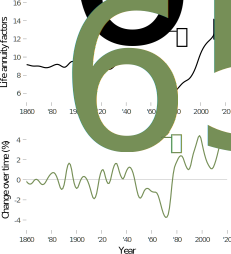
\includegraphics[scale=1.2] {Fig/axm.pdf}
\end{figure}
\end{frame}

\section{Changes over time and sensitivities}

\begin{frame}{Changes over time and sensitivities. Males, 1841-2018}
\begin{figure}
	\centering
	\hspace*{-0.8cm}
	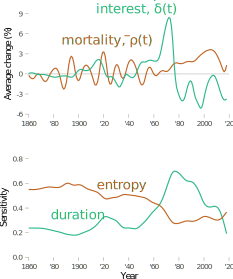
\includegraphics[scale=1.1] {Fig/IntMort.pdf}
\end{figure}
\end{frame}


\section{Assuming a single $\delta(t)$}


\begin{frame}{Decomposition of $\acute{\bar{a}}_x(t)$ at age 65. Males, 1841-2018}
\begin{figure}
	\centering
	\hspace*{-0.9cm}
	\includegraphics[scale=1.2] {Fig/DescSingle0.pdf}
\end{figure}
\end{frame}

\begin{frame}{Decomposition of $\acute{\bar{a}}_x(t)$ at age 65. Males, 1841-2018}
\begin{figure}
	\centering
	\hspace*{-0.9cm}
	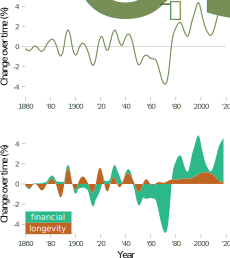
\includegraphics[scale=1.2] {Fig/DescSingle.pdf}
\end{figure}
\end{frame}



\section{Age and term attribution}




\begin{frame}{Age and term attribution. Males, 1970-2018}
\begin{figure}
	\centering
	\hspace*{-0.9cm}
	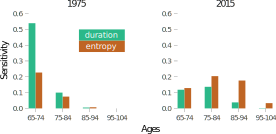
\includegraphics[scale=1.5] {Fig/AttributionDH.pdf}
\end{figure}
\end{frame}


\section{Causes of death}


\begin{frame}{Cause of death attribution}
\begin{figure}
	\centering
	\hspace*{-0.9cm}
	\includegraphics[scale=1] {Fig/DescCod.pdf}
\end{figure}
\end{frame}


\section{To sum up}

\begin{frame}{To sum up}

\textbf{Bringing both perspectives together} \pause
\begin{center}
	\scalebox{2}{$\acute{\bar{a}}_x(t) = \underbrace{\bar{\upvarphi}(t){D}_x(t)}_\text{financial component}+\underbrace{\bar{\rho}(t){H}_x(t)}_\text{longevity component}
		$}\pause
\end{center}
\textbf{Changes over time} in $\bar{a}_x(t)$ are driven by $\dot{\delta}(t)$ and $\bar{\rho}(t)$, which are \textbf{modulated} by  ${D}_x(t)$ and ${H}_x(t)$. \pause


Thorough risk assessment: \textbf{sources of change}\\
$\rightarrow$ Age-term attribution, causes of death, single $\delta(t)$, \\ \pause
 $\rightarrow$ better \textbf{hedging strategies.} \pause

\textbf{No assumptions about the functional form of $\delta$ and $\mu$ (data-driven).}



\end{frame}




\begin{frame}{To sum up}

\textbf{Historical developments in the UK}
\begin{itemize}
	\item \textbf{Longevity risk} has, most of the time, contributed to \textbf{increase} in $\bar{a}_x(t)$, but during some periods it has been \textbf{masked by high financial risk}. \pause
	\item Since the 1980s, \textbf{longevity risk contributes} to most of the increases in $\bar{a}_x(t)$. \pause
	\item \textbf{At higher ages} (i.e. age 75 or older ages): \pause
	\begin{itemize}
		\item The sensitivity of $\bar{a}_x(t)$ to $\mu$ is higher, \pause
		\item Policies aiming at \textbf{increasing retirement ages entail higher longevity risk} (e.g. Denmark, Alvarez et al (2021)).
\end{itemize}
\end{itemize}
\end{frame}

\section{Next steps}

\begin{frame}{Next steps}

\textbf{What about the future?}

\begin{itemize}
	\item Forecasting financial and longevity contributions under different models \pause
	\begin{itemize}
		\item $\bar{\rho}(t)$ and $\bar{\upvarphi}(t)$ can be modelled as \textbf{stochastic processes}, \pause
		\item Interest rates: Cox-Ingersol-Ross (CIR), Vasicek, \pause
		\item Mortality rates: CBD, APC, Lee-Carter, SAINT (ATP), or other models with varying mortality improvements. \pause
	\end{itemize} 
\end{itemize}


\textbf{Extensions and applications} \pause
\begin{itemize}
	\item Other life contingent products, \pause
	\item Guarantees; rolling annuities (Jarner and Preisel, 2017)
	\item Natural hedges; negative correlation between $\bar{a}_x$ and $\bar{A}_x$ (Lin and Tsai, 2014, 2020), \pause
	\item Cashflow, state-dependent $H(t)$ and $D(t)$ (Buchardt and M\o ller 2015), \pause
	\item Sources of change in the reserve $V(t)$ in a \textbf{market-consistent framework} (M\o ller and  Steffensen, 2007). 
\end{itemize}


\end{frame}



\begin{frame}{Decomposition}

\textbf{Rate of mortality improvement}

\begin{equation} \label{eq:rho}
\rho(x,t)=-\frac{\frac{\mu(x,t)}{\partial t}}{\mu(x,t)} = - \frac{\dot{\mu}(x,t)}{\mu(x,t)}.
\end{equation}

\textbf{Change in interest rates over time}

\begin{equation} \label{eq:phi}
\upvarphi(s,t)=-\frac{\frac{\delta(s,t)}{\partial t}}{\delta(s,t)} = -\frac{\dot{\delta}(s,t)}{\delta(s,t)}.
\end{equation}

\end{frame}

\begin{frame}{Decomposition}



\textbf{Entropy}

\begin{equation} \label{eq:EntropyP2}
\begin{split}
{H}^{p}_{x}(t) &=  \frac{\int_0^\infty \mu(x+s,t)   {}_s|\bar{a}_x(t) ds}{\bar{a}_x(t)} 
\end{split}
\end{equation}

\textbf{Duration}

\begin{equation}\label{eq:DurationP2}
\begin{split}
{D}^{p}_{x}(t) &= \frac{\int_0^\infty \delta(s,t) {}_s|\bar{a}_x(t)ds} {\bar{a}_x(t)} 
\end{split}
\end{equation}

\end{frame}

\begin{frame}{Decomposition}

\textbf{Time derivative of $\bar{a}_{x}(t)$ }
\begin{equation}\nonumber
\begin{split}
\dot{\bar{a}}_{x}(t) &=  \int_0^\infty \rho(s,t) \mu(s,t){}_s|\bar{a}_x(t) ds +\int_0^\infty  \upvarphi(s,t) \delta(s,t)  {}_s|\bar{a}_x(t) ds\\
&= \int_0^\infty \rho(s,t) {}_sM_x(t)  ds +\int_0^\infty  \upvarphi(s,t) {}_sW_x(t)  ds,
\end{split}
\end{equation}


where ${}_sM_x(t)= \mu(s,t){}_s|\bar{a}_x(t)$ and ${}_sW_x(t)=\delta(s,t)  {}_s|\bar{a}_x(t)$.

\textbf{Relative derivative of $\bar{a}_{x}(t)$ }

\begin{equation}\nonumber
\begin{split}
\acute{\bar{a}}_x(t) = \frac{\dot{\bar{a}}_x(t)}{\bar{a}_x(t)}  = 
\underbrace{\bar{\rho}(t){H}^{p}_x(t)}_\text{longevity component}
+\underbrace{\bar{\upvarphi}(t){D}^{p}_x(t),}_\text{financial component}
\end{split}
\end{equation}


where $\bar{\rho}_x(t)= \frac{\int_0^\infty \rho(x+s,t) {}_sM_x(t)  ds}{\int_0^\infty  {}_sM_x(t)ds}$ and $\bar{\upvarphi}(t)= \frac{\int_0^\infty \upvarphi(s,t) {}_sW_x(t)  ds}{\int_0^\infty {}_sW_x(t) ds}$ 

\end{frame}



\begin{frame}{Interest and mortality rates for males in the UK, 1841-2018}
\begin{figure}
	\centering
	\hspace*{-0.9cm}
	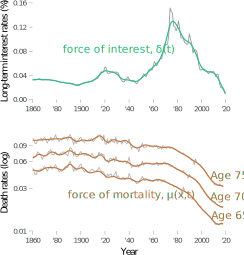
\includegraphics[scale=1.1] {Fig/deltamu.pdf}
\end{figure}
\end{frame}

\begin{frame}{Age and term attribution. Males, 1970-2018}
\begin{figure}
	\centering
	\hspace*{-0.9cm}
	\includegraphics[scale=1.5] {Fig/DescAge.pdf}
\end{figure}
\end{frame}

\end{document}